%        File: topology.tex
%     Created: Thu Nov 09 01:00 PM 2006 C
% Last Change: Thu Nov 09 01:00 PM 2006 C
%
\documentclass[a4paper]{article}
\usepackage{color,graphicx}
\usepackage{amsmath}
\usepackage{amsthm}
\usepackage{amssymb}
\usepackage{amsfonts}
\RequirePackage{ifpdf} % running on pdfTeX?
\ifpdf
\usepackage[pdftex]{hyperref}
\else
\newcommand{\href}[2]{ #1 }
\fi
\title{Netsukuku topology}
\author{http://netsukuku.freaknet.org/}
\begin{document}
\maketitle

\begin{abstract}
	This document describes the fractal structure of the network topology
	of Netsukuku and its practical implementation.
	%%% TODO: aggiungi qualcosa in piu'
\end{abstract}

\section{Preface}
\label{sec:preface}

We're assuming that you already know the basics of the QSPN. If not, read the
QSPN document first: \cite{qspndoc}.

\section{The general idea}
\label{sec:general_idea}

The aim of Netsukuku is to be a (physical) scalable mesh network, completely
distributed and decentralised, anonymous and autonomous.

The software, which must be executed by every node of the net, has to be
unobtrusive. It has to use very few CPU and memory resources, in this way it
will be possible to run it inside low-performance computers, like Access Points,
embedded devices and old computers.

If this requirements are met, Netsukuku can be easily used to build a worldwide
distributed, anonymous and not controlled network, separated from the
Internet, without the support of any servers, ISPs or control authorities.

\section{Basic definitions}

\begin{description}
	\item[Node] We call \emph{node} any computer that is hooked up to the
		Netsukuku network.
	\item[Rnode] stands for remote node: given a node X, it is any other
		node directly linked to X, i.e. it's a neighbour of X.
	\item[Map] A map is a file, kept by each node, which contains all the
		necessary information about the network, f.e. routes and nodes
		status.
\end{description}
Example:\\
\begin{figure}[h]
	\begin{center}
		\includegraphics[scale=0.5]{fig/segABC}
	\end{center}
	\caption{The nodes A,B and C}
\end{figure}
A is the rnode of B.\\
B is the rnode of A and C.\\
C is the rnode of B.

\section{Network topology}
\label{sec:net_topology}

A simple topology, which doesn't impose any structure on the network, can be
memorised with a simple map. In this map, all the information regarding the
nodes of the network have to be memorised. Surely, this kind of map cannot be
utilised by Netsukuku, because it would require too much memory.
For example, even if we store just one route to reach one node and even if
this route costs one byte, we would need 1Gb of memory for a network composed
by $10^9$ nodes (the current Internet).

For this reason, it's necessary to structure the network in a convenient
topology.

\subsection{Fractal topology}
\label{sec:fractal_topology}
\subsubsection{Level 1}
First of all we'll subdivide the network in groups of 256 nodes and we'll use
the following definitions:
\begin{description}
	\item[Gnode] means group node. It is a group of nodes, i.e. a set of
		nodes. Each node of the network belongs to just one gnode.\\
		A gnode contains a maximum of 256 nodes.\\
		By writing $n \in G$ we mean that the node $n$ belongs to the
		gnode $G$.
	\item[Bnode] stands for border node. It is a node which belongs to a
		gnode G, but that is also directly linked to at least one node
		of another gnode, i.e. some of its rnodes belongs to different
		gnodes than its.\\
		By writing $b \in G$ we mean that the bnode $b$ belongs to the
		gnode $G$.
\end{description}

Example:\\
\begin{figure}[h]
	\begin{center}
		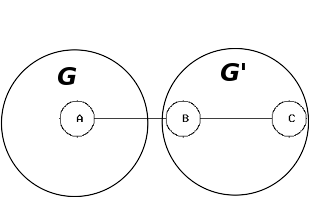
\includegraphics[scale=0.5]{fig/bnode}
	\end{center}
	\caption{The bnode A and B, belonging respectively to the gnode G and
	$G'$}
\end{figure}
$A \in G $, A is a node belonging to the gnode G, its rnode is B.\\
$B \in G'$, B is a node belonging to the gnode $G'$, its rnode is A.\\
A is a bnode of G, while B is a bnode of $G'$.

\subsubsection{Level n}
We further subdivide the network topology in \emph{groups of 256 groups of nodes}
and we continue to name them as gnode.\\
At this point, we repeat recursively this subdivision process until
we can group all the nodes of the network into a single gnode.

Doing so, we've structured the network in $n+1$ levels (from $0$ to $n$).\\
In the base level (level 0), there are 256 single nodes.\\
In the first level (level 1), there are 256 normal gnodes. Each of them
contains 256 single nodes.\\
In the second (level 2), 256 gnodes of level 1 forms a single \emph{group of
groups of nodes}.\\
In the third (level 3), there are 256 groups of 256 groups of 256 groups of
256 nodes.\\
Continuing in this way, we arrive at the last level (level $n$), where there
is a single group which contains the whole network.\\

The QSPN algorithm is able to operate independently on any level,
considering each gnode as a single node of level 0.
For this reason, we can view the Netsukuku topology as a fractal, where each
level is composed by single nodes.

\subsubsection*{Example}

Figure \ref{fig:fract_circle}\footnote{this figure has been taken from:
\href{http://www.ian.org/FX/Plugins.html}{http://www.ian.org/FX/Plugins.html}}
is an example of the fractal topology of Netsukuku.

\begin{figure}[h]
	\begin{center}
		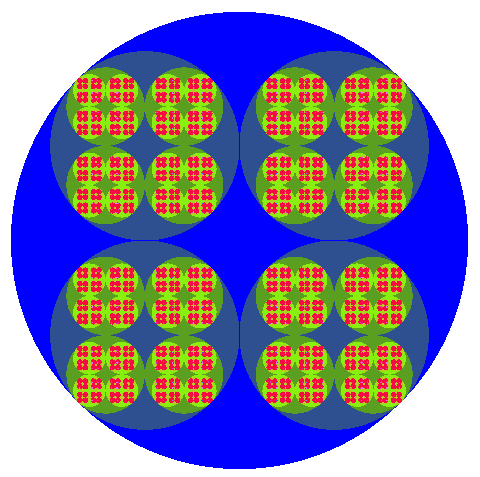
\includegraphics[scale=0.5]{fig/fractal_circle}
	\end{center}
	\caption{An example of the netsukuku topology structure}
	\label{fig:fract_circle}
\end{figure}

In this topology, each gnode contains four nodes, i.e. each group contains
four elements. The network is structured in 5 levels. The red elements, are single
nodes. The bright green circle are groups of nodes. The dark green circles are
groups of groups of nodes. The dark blue circle are groups of groups of groups of
nodes. Finally, the bright blue circle is the gnode which contains the whole
network.

\subsubsection{Membership}
Let's assign a numeric ID to each (g)gnode, starting from the last level:
\begin{enumerate}
	\item in the last level ($n$) there's only one giant gnode, thus we assign
		to it the ID ``0''. Our global ID will be:
		\[
		0
		\]
	\item in $n-1$ there are 256 gnodes, which belongs to the gnode 0 of
		level $n$, thus we assign them the IDs from $0$ to $255$.
		The global ID becomes:
		\[
		0\cdot i\quad 0\le  i\le 255
		\]
	\item we repeat the step 2 recursively gaining an ID of this form:
		\[
		0\cdot i_{n-1}\cdot i_{n-2}\cdot \dots \cdot i_0 \quad 0\le i_j\le 255,\;0\le j\le n-1
		\]
	\item since the last level is always $0$, we'll omit it and we'll
		consider only the first $n$ levels.
\end{enumerate}
In a network with a maximum of $2^{32}$ nodes (the maximum allowed by the ipv4),
there would be five levels ($n=4$), where each gnode will be composed by 256 nodes.
Therefore, the ID will be in the usual IP form:
\[
0\dots255\cdot 0\dots255\cdot 0\dots255\cdot 0\dots255
\]
For example, a single node of level 0 of the network is:
\[
3\cdot 41\cdot 5\cdot 12
\]
That said, each gnode of the network belongs to only one combination of gnodes
of the various levels. In our previous example we have:
\begin{align*}
	&g_3=3\\
	&g_2=41\\
	&g_1=5\\
	&g_0=12
\end{align*}
where each $g_i$ corresponds to the gnode ID of the level $i$. Note that $g_0$
is the ID attributed to the single node, at level 0.

\subsection{Fractal map}
The advantages of using a fractal topology are clear.\\
The node $N$, instead of memorising information about each node of the whole
network, will keep only that regarding the gnodes where it belongs to.
Suppose the node $N$ had this ID:
\[
g_3\cdot g_2\cdot g_1\cdot g_0
\]
It will store in memory information regarding:
\begin{enumerate}
	\item the 256 single nodes which belongs to its same gnode of level 1,
		or in other words, the 256 nodes of the gnode $g_1$,
	\item the 256 gnodes gnodes which belongs to its same gnode of level
		2, of in other words, the 256 gnodes of the gnode $g_2$,
	\item finally, the 256 gnodes which belongs to the gnode $g_3$.
\end{enumerate}
Note that doing so, the node $N$ will be blind to all the other gnodes. For
example, it won't know any information regarding the single nodes which belong
to all the other gnodes of level 1 different from $g_1$.\\

Even with this lack of knowledge, as we'll see later, the node $N$ is still
able to reach all the other nodes of the network.
In conclusion, $N$ only needs $256n$ entries in its map, instead of $2^{32}$. 
To clarify the ideas suppose that each entry costs one byte. In the plain
topology we needed $4Gb$, while in the fractal one we just need $256\cdot 4\;
b= 1Kb$.

\subsubsection{IP v4 and v6}
Netsukuku is both compatible with ipv4 and ipv6.\\

In ipv4 there are a maximum of $2^{32}$ IPs, thus we have five levels $n=4$.\\
In ipv6 there are a maximum of $2^{128}$ IPs, thus $n=16$.

\subsubsection{Internal and external map}
For simplicity we divide the map of the node $N$, in the \emph{internal map} and in
the \emph{external} one.  The internal map contains information regarding the
nodes belonging to $g_1$. The external map describes all the other levels of
the topology.

\subsubsection{Bnode map}
The bnode map of the node $N$  contains the information regarding the bnodes
of each level where $N$ belongs.
Some examples to clarify the ideas:\\

suppose that $N = g_3\cdot g_2\cdot g_1 \cdot g_0$
\begin{itemize}
	\item a bnode of level 0 is a single node linked with two nodes of two
		different gnodes of level 1.
	\item the bnodes of level 0, known by $N$, are only that which belong
		to the gnode $g_0$. Thus are all the nodes of $g_0$ which are
		linked to at least a gnode different from $g_1$.
\end{itemize}

\subsection{CIDR routing}
The QSPN, for each level, will build the routes necessary to connect each
(g)node to all the other (g)nodes of the same level. The routes will be saved
in the maps of each node.\\

If the node $N=g_3\cdot g_2\cdot g_1 \cdot g_0$ wants to reach a node $M$ which
belongs to different gnodes, f.e. $M=g_3\cdot g_2\cdot h_1 \cdot h_0$, it will
add a CIDR\cite{CIDR} route in the routing table of the kernel:\\
\emph{all the packets whose destination is $g_3\cdot g_2\cdot h_1 \cdot 0\dots
255$ will be forwarded to the gateway $X$}.\\

We'll see later how the gateway $X$ is chosen.

\subsection{Tracer Packets in high levels}
In the QSPN document \cite{qspndoc}, we've seen how a Tracer Packet works in a
network composed by single nodes, i.e. a gnode of level 0. \\
We'll now study its way of working on higher levels.

\subsubsection{A gnode is a node}
In the abstract sense a single node is an entity which:
\begin{enumerate}
	\item receives input from its links
	\item stores it in its memory
	\item computes it
	\item and sends the output of the computation over some of its links
\end{enumerate}
Thus any other entity which performs the same operations can be thought as a
single node.\\
A gnode $G$ can act as a single node too.
\begin{enumerate}
	\item A bnode $I$, which belongs to $G$, receives an input from its
		links. We call $I$ the ingress (b)node.
	\item this input is flooded to all the nodes, of any level, of the
		gnode. The nodes will memorize the information contained in
		the input.\\
		Note that the flood is not a TP. The flooded pkt will be
		received only once by each node.
	\item A bnode $O$, of the same gnode, which is different from $I$,
		receives the flooded input and computes it.
		We call $O$ the egress (b)node.
	\item The bnode $O$ sends the output of its computation to its
		external links, i.e. avoiding those links which connect it to
		nodes of $G$ or to the same gnode which sent the input to $I$.
\end{enumerate}

\subsubsection{Example of a wandering TP}
Consider the network in figure \ref{fig:qspn_g3}.\\
\begin{figure}[h]
	\begin{center}
		\includegraphics[scale=0.5]{fig/qspn_g3}
	\end{center}
	\caption{The gnodes $G_1$, $G_2$ and $G_3$}
	\label{fig:qspn_g3}
\end{figure}
$G_1$, $G_2$, $G_3$ are gnodes of level 1. $A_1$ and $A_2$ belong to $G_1$. $B_1$ and $B_2$ belong to
$G_2$. $C_1$ belongs to $G_3$.\\

Suppose the node $A_1$ sends a Tracer Packet in level 1 
\footnote{Note that any node can send a TP in any level. In this case, we are
considering $A_1$, which is a bnode, to simplify the example}. 
The following will happen:
\begin{enumerate}
	\item The TP is flooded in $G_1$.
	\item $A_2$ receives the TP and appends in it the ID of the gnode
		$G_1$.
	\item $A_2$ sends the TP to $B_1$.
	\item $B_1$ receives it, updates its maps and floods it in $G_2$.
	\item All the node belonging to $G_2$ will receive the TP, updating their
		maps.
	\item This same procedure is reiterated from step 2, i.e. $B_2$ receives
		the TP, appends the ID of $G_2$ and so on until $C_1$ receives
		it.
	\item $C_1$, noticing that its gnode hasn't any links to other gnodes
		than $G_2$, will bounce back the TP to $B_2$ and at the same
		time will flood $G_3$.
	\item The TP, with the same procedure, will return back to $A_1$,
		completing the TP cycle.
\end{enumerate}

\subsection{QSPN v2 in high levels}
In order to use the $Q^2$ (QSPN v2) in high levels, we need to be sure that a TP,
flooded inside a lower gnode, will reach once and only once all the nodes of
the same gnode. Moreover, a good metric needs to be defined for the high
levels: what is the rtt (Round-Trip Time) and bandwidth capacity of the link
between the two gnodes $G_1$ and $G_2$?

\subsubsection{Unique flood}
The first requirement is easily solvable.\\

Suppose that a TP has been flooded inside the gnode $G$.
Suppose also that the node $N$ of $G$ receives two duplicate packets.\\
The $Q^2$ instructs the node $N$ to keep forwarding only the interesting packets.
A packet, which is a perfect copy of a packet already received, is always
uninteresting. Therefore, the node $N$ will drop the second copy of the
received TP.\\

Whenever two or more copies of a same TP are received by a node
of $G$, only one of them will be forwarded. Hence, the successive nodes will
receive only one copy of the same packet.

\subsubsection{Endless loops}
Consider the situation in figure \ref{fig:3bnodes}.
\begin{figure}[h]
	\begin{center}
		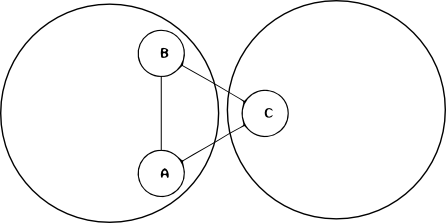
\includegraphics[scale=0.6]{fig/3bnodes}
	\end{center}
	\caption{Three bnodes, forming a cycle}
	\label{fig:3bnodes}
\end{figure}
A and B are bnodes of the node $G_1$, while $C$ is a bnode of the gnode $G_2$.
Suppose C sends a TP to B. B floods it inside $G_1$, thus $A$ receives it. At
this point, $A$ sends the packet to all its external links, and thus to $C$.
$C$ will send the packet again to $B$ and the cycle will continue.\\

This situation can be avoided if an ingress bnode, before forwarding a packet to a an
external gnode $F$, checks if the packet has already traversed $F$ itself. If
it has, the bnode won't forward it to $F$.

\subsubsection{Gnode metric}
We will refer to REM (Route Efficiency Measure), as a value characterising the
quality of a route. REM can be calculated in various ways, f.e. by taking in
account the total rtt and the bw capacity of the route. We suppose that
the REM value of a normal route/link has been already defined. The REM value
of a route, whose hops are gnodes and single nodes is defined as follow.
\begin{enumerate}
	\item The REM value of the route $x\rightarrow y$ is $E(x\rightarrow
		y)$.
	\item Let $G$ be a gnode, $x$ one of its nodes and $x \rightarrow G$ the
		link between the node and the gnode. $x \rightarrow G$ can be
		thought as the set of all the routes, which connect $x$ to
		each node of $G$. The REM value of $x \rightarrow G$, should
		tell the ability of the node $x$ to reach a generic node of
		$G$. For this reason, we define $E(x \rightarrow G)$ as the
		aritmetic mean of the REM value of all the routes, connecting
		$x$ to every node of $G$. In symbols:
		\[
		\begin{matrix}
			n=|G|,\quad g_i\in G\\
		E(x\rightarrow G)=\frac{\sum_{i=1}^n E(x \rightarrow g_i)}{n}
		\end{matrix}
		\]
		where $g_i$ is a node of $G$, and $n$ is the number of nodes
		of $G$.
	\item Let $G$ be a gnode, $g_i' \in G$ its $i$-th bnode. Let $H$ be a
		gnode bordering with $G$, $x \in H$ one of its nodes, and
		$h_j' \in H$ its $j$-th bnode. Finally let
		$\{g_1',\dots,g_j'\}$ be the set of the bnodes of $G$ which
		are connected respectively with $h_1', h_2', \dots$.\\
		The REM value of the link $x\rightarrow G$ is calculated as
		follow:
		\begin{eqnarray*}
		E(x \rightarrow \{g_1',\dots,g_j'\})&=&\frac{\sum_{i=1}^j
		E(x \rightarrow h_i' \rightarrow g_i')}{j}\\
		E(\{h_1',\dots,h_j'\}\rightarrow G)&=&\frac{\sum_{i=1}^j
		E(h_i'\rightarrow G)}{j}\\
		E(x\rightarrow G)&=&\frac{E(x \rightarrow
		\{g_1',\dots,g_j'\})+E(\{h_1',\dots,h_j'\}\rightarrow G)}{2}
		\end{eqnarray*}
\end{enumerate}


Each link contained in a TP contains its relative REM value. For example, in
the TP $I \rightarrow B \rightarrow  C$, there will be the REM values for $I
\rightarrow B$ and $B\rightarrow C$. In the following example, we'll show how
the REM values are computed and inserted in the TP.\\

Consider the network in figure \ref{fig:gmetric}.
%%%%%%%% TODO G_3 \rightarrow  G_2
Suppose that $G_3$ sent a TP.\\
When the ingress bnode $B_i \in G_2, \;i=1,2,3$ receives the TP it will
calculate the following REM value, appending it in the packet:
\[
REM(G_3\rightarrow G_2) = 
\]
of $B_i \rightarrow  C_i$
Suppose that the egress bnode $A_2$ of the gnode $G_2$ received the TP $G_3
\rightarrow  G_2$\\
The bnode $A_2$ calculates the REM value of the last link appended ($G_3
\rightarrow  G_2$) in the packet and adds it in the packet itself.
The REM value is calculated as follow:
\[
REM(G_3\rightarrow G_2) = 
\]

%%%%%%%%% TODO: continue here 
\begin{figure}[h]
	\begin{center}
		\includegraphics[scale=0.4]{fig/gmetric}
	\end{center}
	\caption{Gnodes metric example}
	\label{fig:gmetric}
\end{figure}

%%%%%%%%%%%%%%%%%%%%  TODO %%%%%%%%%%%%%%%%%%%%%

%%%% Q^2 pseudocode for high levels:
%%%%  bnode_receive(),  node_receive()
%
% Per droppare i DUP non bisogna considerare il REM ma solo gli hop the TP!!!!
%
%bnode map
%	Size
%ext map  (sizeof)
%int map	(sizeof)
%QSPN per livelli alti: chi manda chi e cosa
%			specificare i casi in cui viene mandato un Q nei
%			livelli alti
%
%Radar: quand'e' che viene mandata un Q2.
% 	Delay di attesa prima di mandare il Q2.

%%%%%%%%%%%%%%%%
% Bibliography %
%%%%%%%%%%%%%%%%

\begin{thebibliography}{99}
	\bibitem{qspndoc} QSPN document:
		\href{http://netsukuku.freaknet.org/doc/main\_doc/qspn.pdf}{qspn.pdf}
	\bibitem{ntksite} Netsukuku website:
		\href{http://netsukuku.freaknet.org/}{http://netsukuku.freaknet.org/}
	\bibitem{CIDR} CIDR routing:
		\href{http://en.wikipedia.org/wiki/Classless\_Inter-Domain\_Routing}{Classless\_Inter-Domain\_Routing in Wikipedia}
\end{thebibliography}
\newpage

\begin{center}
\verb|^_^|
\end{center}
\end{document}
